%!TeX program = xelatex
\documentclass[12pt,hyperref,a4paper,UTF8]{ctexart}
\usepackage{HDUReport}
\usepackage{listings}
\usepackage{xcolor}
\usepackage{graphicx}
\usepackage{setspace}
\usepackage{float}
\setstretch{1.5} % 设置全局行距为1.5倍

\usepackage{enumitem} % 载入enumitem包以便自定义列表环境
\setlist[itemize]{itemsep=0pt, parsep=0pt} % 设置itemize环境的项目间距和段落间距

\setmainfont{Times New Roman} % 英文正文为Times New Roman

%封面页设置
{   
    %标题
    \title{ 
        \vspace{1cm}
        \heiti \Huge \textbf{Linux系统及应用作业报告} \par
        \vspace{1cm} 
        \heiti \Large {\underline{作业3:文件时间}   } 
        \vspace{3cm}
    
    }

    \author{
        \vspace{0.5cm}
        \kaishu\Large 学院\ \dlmu[9cm]{卓越学院} \\ %学院
        \vspace{0.5cm}
        \kaishu\Large 学号\ \dlmu[9cm]{23040447} \\ %班级
        \vspace{0.5cm}
        \kaishu\Large 姓名\ \dlmu[9cm]{陈文轩} \qquad  \\ %学号
        \vspace{0.5cm}
        \kaishu\Large 专业\ \dlmu[9cm]{智能硬件与系统(电子信息工程)} \qquad \\ %姓名 
    }
        
    \date{\today} % 默认为今天的日期,可以注释掉不显示日期
}
%%------------------------document环境开始------------------------%%
\begin{document}

%%-----------------------封面--------------------%%
\cover
\thispagestyle{empty} % 首页不显示页码
%%------------------摘要-------------%%
%\newpage
%\begin{abstract}




%\end{abstract}

%\thispagestyle{empty} % 首页不显示页码

%%--------------------------目录页------------------------%%
% \newpage
% \tableofcontents
% \thispagestyle{empty} % 目录不显示页码

%%------------------------正文页从这里开始-------------------%
\newpage
\setcounter{page}{1} % 让页码从正文开始编号

%%可选择这里也放一个标题
%\begin{center}
%    \title{ \Huge \textbf{{标题}}}
%\end{center}

\section{问题1}
\textbf{"Access Time"中的"Access"是指哪种操作?设计一个示例,操作演示一下Access Time的变化。}

\subsection{Access Time 定义}
在Linux系统中,"Access Time"(访问时间,简称 atime)指的是文件最后一次被\textbf{读取}或\textbf{执行}的时间。这包括但不限于以下操作:
\begin{itemize}
    \item 使用 \texttt{cat}, \texttt{less}, \texttt{head} 等命令查看文件内容
    \item 程序读取文件内容
    \item 执行脚本文件
\end{itemize}

\subsection{示例演示}
\begin{lstlisting}[language=bash, caption=演示Access Time变化]
# 1. 创建测试文件并查看初始时间戳
echo "This is a test file." > testfile.txt
stat testfile.txt

# 2. 访问文件内容
cat testfile.txt

# 3. 再次查看时间戳,观察Access Time变化
stat testfile.txt
\end{lstlisting}

\subsection{预期结果}
\begin{itemize}
    \item 第一次 \texttt{stat} 命令输出中的 Access Time 显示文件创建时间
    \item 执行 \texttt{cat} 命令后,Access Time 更新为执行 \texttt{cat} 时的时间
    \item Modify Time 和 Change Time 保持不变
\end{itemize}

\subsection{实际结果}

\begin{figure}[H] % [H] 表示强制当前位置插入
    \centering
    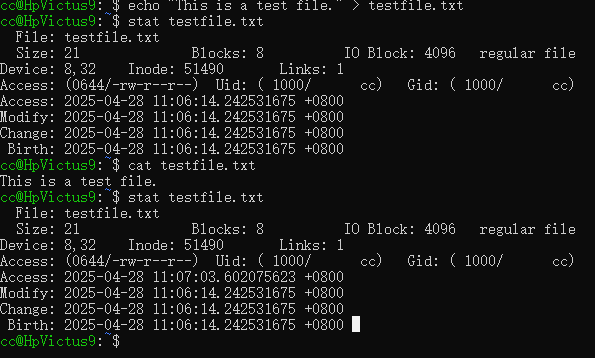
\includegraphics[width=0.8\textwidth]{figures/L1.png} % 调整宽度为文本宽度的 80%
    \caption{WSL实际测试效果} % 图片标题
    \label{fig:example} % 图片标签,用于引用
\end{figure}

可以发现,只有Access Time时间变化,Modify Time 和 Change Time 保持不变,符合预期。


\section{问题2}
\textbf{设计一个示例,演示"Modified Time"和"Change Time"的区别。}

\subsection{时间戳区别}
\begin{itemize}
    \item \textbf{Modified Time (mtime)}: 文件内容最后一次被修改的时间
    \item \textbf{Change Time (ctime)}: 文件元数据(权限、所有者等)或内容被修改的时间
\end{itemize}

\subsection{示例演示}
\begin{lstlisting}[language=bash, caption=演示mtime和ctime区别]
# 1. 创建文件并记录初始时间戳
echo "Initial content" > demo.txt
stat demo.txt

# 2. 修改文件内容(会更新mtime和ctime)
echo "Modified content" > demo.txt
stat demo.txt

# 3. 仅修改文件权限(只更新ctime)
chmod 600 demo.txt
stat demo.txt
\end{lstlisting}

\subsection{预期结果}
\begin{center}
\begin{tabular}{|l|c|c|}
\hline
操作 & Modified Time & Change Time \\
\hline
初始创建 & T1 & T1 \\
修改内容 & T2 & T2 \\
修改权限 & T2 & T3 \\
\hline
\end{tabular}
\end{center}

其中T1 < T2 < T3,表明:
\begin{itemize}
    \item 修改内容会同时更新mtime和ctime
    \item 修改权限只会更新ctime
\end{itemize}

\subsection{实际结果}

\begin{figure}[H] % [H] 表示强制当前位置插入
    \centering
    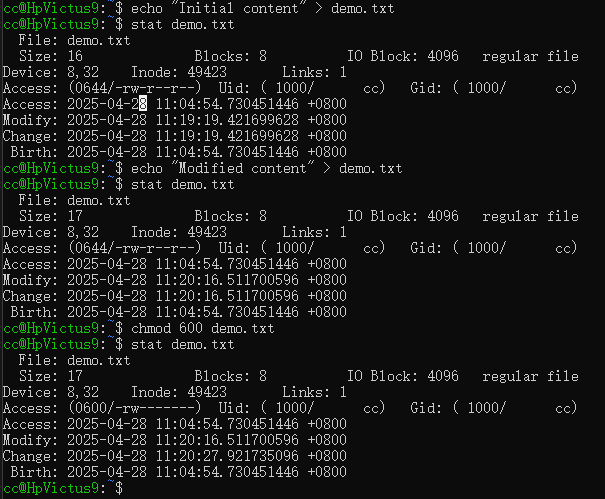
\includegraphics[width=0.8\textwidth]{figures/L2.png} % 调整宽度为文本宽度的 80%
    \caption{WSL实际测试效果} % 图片标题
    \label{fig:example} % 图片标签,用于引用
\end{figure}

可以发现,执行第二个“echo "Modified content" > demo.txt”(修稿文件内容指令),Modified Time 和 Change Time
都有更改。“chmod 600 demo.txt”(更改文件权限,使文件所有者可读写,其他用户无权限)指令执行后,只有Change Time更新。

\end{document}

